\documentclass[10pt,a4paper]{standalone}
\usepackage{amssymb}
\usepackage{amsmath}
\usepackage{bm}
\usepackage{tikz}
\usetikzlibrary{arrows.meta}
\usetikzlibrary{arrows}
\usepackage{pstricks}
\usetikzlibrary{patterns}
\usetikzlibrary{fadings}
\usetikzlibrary{shapes.geometric}


\begin{document}
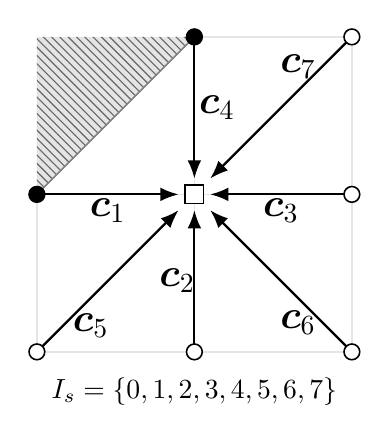
\begin{tikzpicture}[line width=0.2mm]
	\def\rstart{0.2}   % distance from center
	\def\rlen{1.8}      % arrow length

\fill[gray!20] (4,4) -- (4,6) -- (6,6) -- cycle;
\fill[pattern=north west lines, pattern color=black!60] (4,4) -- (4,6) -- (6,6) -- cycle;

\draw[solid,thin,line width=0.2mm, black!50 ] (4,4) -- (6,6);
%\fill[gray!40] (4,4) -- (8,4) -- (8,6) -- (4,6) -- cycle;
%\fill[gray!40] (6,2) -- (8,2) -- (8,4) -- (6,4) -- cycle;

%\draw[dashed,thin,line width=0.1mm] (3.5,4) -- (8.5,4);

\draw[solid,thin,line width=0.2mm, gray!20] (4,2) -- (8,2);
\draw[solid,thin,line width=0.2mm, gray!20] (4,4) -- (8,4);
\draw[solid,thin,line width=0.2mm, gray!20] (6,6) -- (8,6);

\draw[solid,thin,line width=0.2mm, gray!20] (6,2) -- (6,6);
\draw[solid,thin,line width=0.2mm, gray!20] (8,2) -- (8,6);
\draw[solid,thin,line width=0.2mm, gray!20] (4,2) -- (4,4);

\draw[black, thick, {Latex}-]
(6,4) ++(\rstart,0) -- ++(\rlen,0)
node[midway,below, yshift=2pt,font=\fontsize{14pt}{12pt}\selectfont] {$\bm{c}_3$};

% up (2)
\draw[black, thick, {Latex}-]
(6,4) ++(0,\rstart) -- ++(0,\rlen)
node[midway, right, xshift=-2pt,font=\fontsize{14pt}{12pt}\selectfont] {$\bm{c}_4$};

% left (3)
\draw[black, thick, {Latex}-]
(6,4) ++(-\rstart,0) -- ++(-\rlen,0)
node[midway, below, yshift=2pt,font=\fontsize{14pt}{12pt}\selectfont] {$\bm{c}_1$};

% down (4)
\draw[black, thick, {Latex}-]
(6,4) ++(0,-\rstart) -- ++(0,-\rlen)
node[midway, left, xshift=4pt,font=\fontsize{14pt}{12pt}\selectfont] {$\bm{c}_2$};

\draw[black, thick, {Latex}-]
(6,4) ++(-\rstart,-\rstart) -- ++(-\rlen,-\rlen)
node[midway, below left,xshift=4pt, yshift=-8pt,font=\fontsize{14pt}{12pt}\selectfont] {$\bm{c}_5$};

% diagonals
\draw[black, thick, {Latex}-]
(6,4) ++(\rstart,\rstart) -- ++(\rlen,\rlen)
node[midway, above right,xshift=-4pt, yshift=7pt,font=\fontsize{14pt}{12pt}\selectfont] {$\bm{c}_7$};

\draw[black, thick, {Latex}-]
(6,4) ++(\rstart,-\rstart) -- ++(\rlen,-\rlen)
node[midway, below right,xshift=-4pt, yshift=-7pt,font=\fontsize{14pt}{12pt}\selectfont] {$\bm{c}_6$};

%\draw[black, thick, {Latex}-]
%(6,4) ++(-\rstart,\rstart) -- ++(-\rlen,\rlen)
%node[midway, above left,xshift=4pt, yshift=7pt,font=\fontsize{14pt}{12pt}\selectfont] {$\bm{c}_8$};

%\draw (5.6,4.6)node[]{$\mathbf{0}$};
%\draw (8.3,4.3)node[]{$\mathbf{1}$};
%\draw (6.3,6.3)node[]{$\mathbf{2}$};
%\draw (3.7,4.3)node[]{$\mathbf{3}$};
%\draw (5.7,1.7)node[]{$\mathbf{4}$};
%\draw (8.3,6.3)node[]{$\mathbf{5}$};
%\draw (3.7,6.3)node[]{$\mathbf{6}$};
%\draw (3.7,1.7)node[]{$\mathbf{7}$};
%\draw (8.3,1.7)node[]{$\mathbf{8}$};

\node[draw, black, fill=white, rectangle, minimum size=0.2cm] at (6,4) {};
%\draw[black,fill=black] (6,4)node[]{} circle(0.1cm); %0
\draw[black,fill=white] (8,4)node[]{} circle(0.1cm);%1
\draw[black,fill=white] (6,2)node[]{} circle(0.1cm);%2
\draw[black,fill=black] (4,4)node[]{} circle(0.1cm);%3
\draw[black,fill=black] (6,6)node[]{} circle(0.1cm);%4
\draw[black,fill=white] (8,6)node[]{} circle(0.1cm);%5
%\draw[black,fill=white] (4,6)node[]{} circle(0.1cm);%6
\draw[black,fill=white] (4,2)node[]{} circle(0.1cm);%7
\draw[black,fill=white] (8,2)node[]{} circle(0.1cm);%8


\draw (6,1.5)node[]{$I_s = \{0,1,2,3,4,5,6,7\}$};
%\draw (6,1)node[]{$O_s = \{0,1,2,3,4,5,7,8\}$};


\end{tikzpicture}
\end{document}



